\section{Systematic Studies}
Systematic uncertainties are discussed in this section. 
Variation in specific cuts may affect the result. Due to a
large variation of statistical uncertainty involved in this analysis, 
a point to point systematic approach is not realistic. Therefore, 
an estimation on the systematic errors is made varying each cut 
and taking the average relative difference in the final result. 
The systematic uncertainty is quoted based as the shift of the 
average of the relative differences from zero. The average values
are ``Mean'' values shown in the statistical box of each relative difference plot.
The relative difference is given by
\begin{equation}
 Relative~Difference = \frac{R_{Nominal} - R_{variation}}{R_{Nominal}}
\end{equation}
where $R_{Nominal}$ is the differential cross section quoted and $R_{variation}$ 
is the differential cross section (unless mentioned otherwise in the text) 
calculated by varying any specific cut. The systematic uncertainties 
are discussed in the following sections.

\subsection{Fitting function}
\label{Sec:SysSecDep}
This includes the systematic effect based on different modules/sectors of the PCAL. The systematic
studies are completed for all modules/sectors with their respective runs to analyze the effect
upon switching to Landau function from Gaussian function to fit the signal.

Nominally, the ADC distribution is fit using a Gaussian function. The fit function was changed to
a Landau function which also has three parameters similar to that of a Gaussian function. The events
undergo similar fitting procedure after the centroids are extracted. Both sets of attenuation coefficients
are then compared. As there are three coefficients, the gain ($A+C$) is used to compare. An average systematic effect for this variation for all layers and all sectors is found to
be $\sim7\%$. For each module and layer, the systematic variation is summarized in Table~\ref{sysTab1}.
For run 4416 (Module 6, Sector 5), the systematic variation for U-layer is shown in Fig.~\ref{fig:lanVgaus4416}.

\FloatBarrier
\begin{table}[h]
        \centering{}
        \scalebox{1.0}{
	\begin{tabular}{|c|c|c|c|c|c|c|c|c|c|c|c|}
	\hline
\multirow{2}{*}{Module} & \multirow{2}{*}{Sector} & \multirow{2}{*}{Run} & \multicolumn{3}{c|}{Systematics U-strip (\%)}        & \multicolumn{3}{c|}{Systematics V-strip (\%)}         & \multicolumn{3}{c|}{Systematics W-strip (\%)}          \\ \cline{4-12} 
                        &                         &                      & run  & average               & U-strip               & run   & average               & V-strip               & run   & average                & W-strip               \\ \hline
\multirow{2}{*}{1}      & \multirow{2}{*}{4}      & 4103                 & 1.64 & \multirow{2}{*}{1.76} & \multirow{8}{*}{3.92} & 1.76     & \multirow{2}{*}{6.69} & \multirow{8}{*}{10.35} & 29.44 & \multirow{2}{*}{21.56} & \multirow{8}{*}{7.24} \\ \cline{3-4} \cline{7-7} \cline{10-10}
                        &                         & 4108                 & 1.89 &                       &                       & 12.95 &                       &                       & 13.68 &                        &                       \\ \cline{1-5} \cline{7-8} \cline{10-11}
2                       & 3                       & 4167                 & 9.66 & 9.66                  &                       & 36.17 & 36.17                 &                       & 13.61 & 13.61                  &                       \\ \cline{1-5} \cline{7-8} \cline{10-11}
3                       & 2                       & 4250                 & 6.31 & 6.31                  &                       & 16.95 & 16.95                 &                       & 2.47  & 2.47                   &                       \\ \cline{1-5} \cline{7-8} \cline{10-11}
\multirow{2}{*}{4}      & \multirow{2}{*}{1}      & 4285                 & 2.90 & \multirow{2}{*}{2.21} &                       & 0.17  & \multirow{2}{*}{0.32} &                       & 3.00  & \multirow{2}{*}{2.20}  &                       \\ \cline{3-4} \cline{7-7} \cline{10-10}
                        &                         & 4289                 & 1.53 &                       &                       & 0.47  &                       &                       & 1.39  &                        &                       \\ \cline{1-5} \cline{7-8} \cline{10-11}
5                       & 6                       & 4294                 & 3.04 & 3.04                  &                       & 1.45  & 1.45                  &                       & 2.34  & 2.34                   &                       \\ \cline{1-5} \cline{7-8} \cline{10-11}
6                       & 5                       & 4416                 & 0.51 & 0.51                  &                       & 0.54  & 0.54                  &                       & 1.26  & 1.26                   &                       \\ \hline
	\end{tabular}
        }
	\label{sysTab1}
        \caption{Sytematics for the attentuation co-efficients.}
\end{table}

\begin{figure}[h]
  \centering
  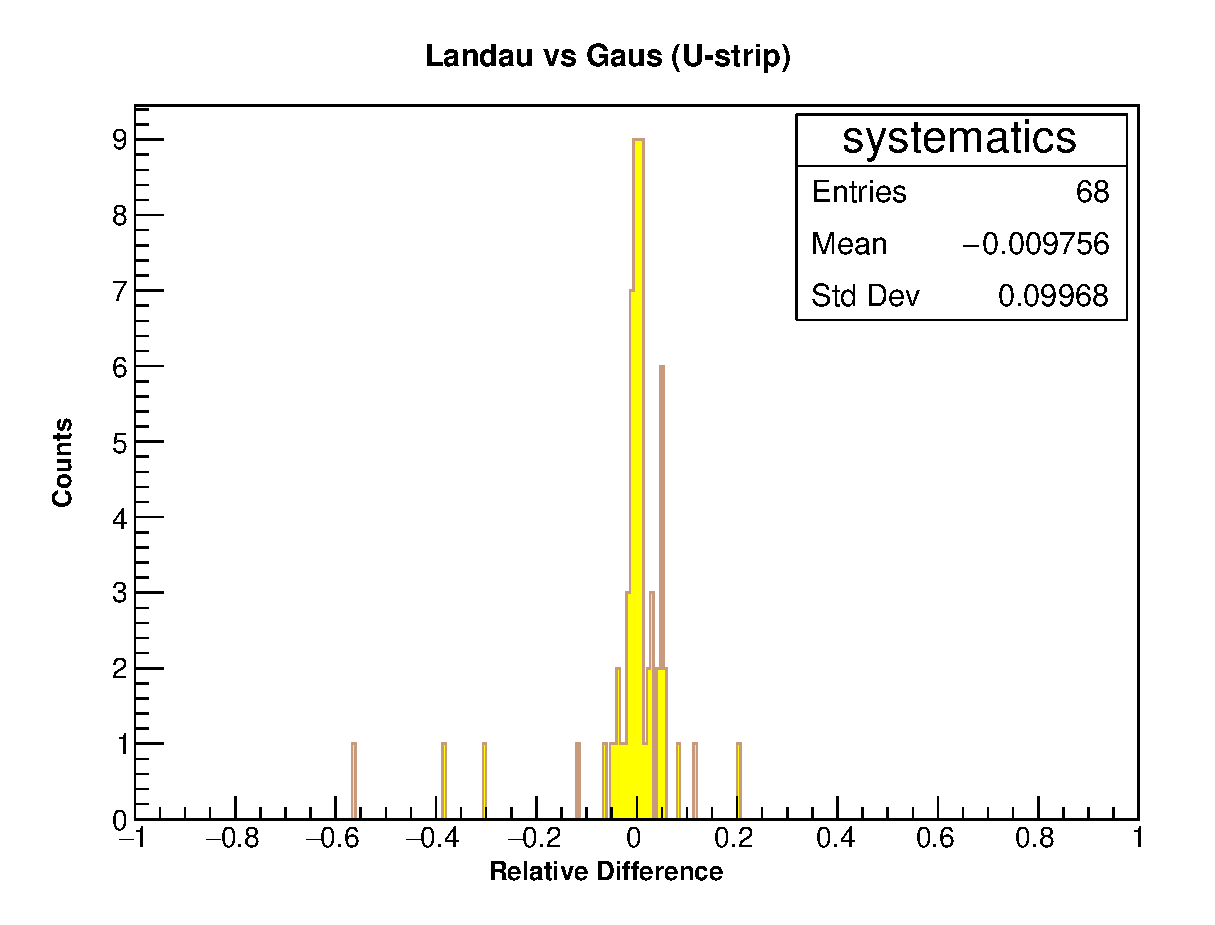
\includegraphics[width=\textwidth, height = 2.5in, keepaspectratio = true]{lanVgausU-mod6sec5-4416}
  \caption{Shown in the systematic effect in the gain when using a Landau function over all passes relative to when using a Gaussian function for U-layers in run 4416.}
  \label{fig:lanVgaus}
  % plot created using /home/chetry/EC_PCAL/PCALanalysis_inC_taya/com/sys.c
\end{figure}

